\newpage
\chapter{Experiments and Results}
\label{sec:ExperimentsandResults}
In order to test the previously described \ac{TAD} approach several experiments were performed, to find the optimal model for both the \ac{SISR} and \ac{IC} tasks, to show the impact of the L1 ball on the model's robustness against perturbations as well as evincing the feasibility of applying the \ac{TAD} method in the video domain.

\begin{figure}[!htbp]
	\centering
	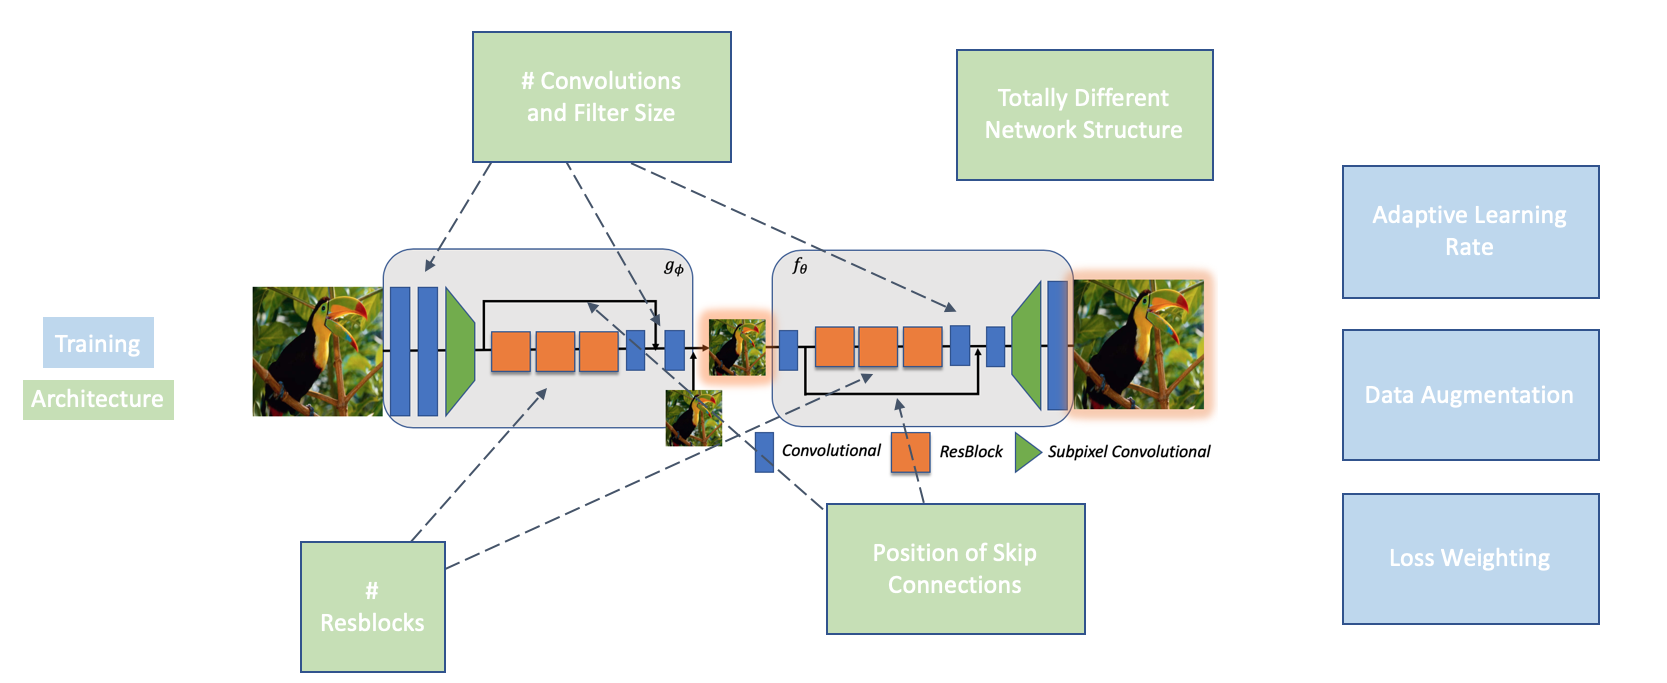
\includegraphics[width=14cm]{figures/model_adaptions}
	\caption{Model and Training adaptions during experiments in comparison
  to the baseline model by \cite{TAID}.}
  \label{fig:model_adaptions}
\end{figure}

As shown in \myfigref{fig:model_adaptions} a bunch of adjustments to the
baseline model (by \cite{TAID}) were tried for analyzing the coherence between the model complexity and its reconstruction performance. Thereby very small architectures (6 layers) as well as comparable large architectures (19 layers) were tested (baseline model has 10 layers), spanning from $375.926$ to $1.299.126$ parameters. Since the model already is quite shallow the removal of each layer had an impact on the resulting performance, therefore especially the number of \textit{Resblocks} (two convolutional layers and ReLU) has a huge impact on the reconstruction accuracy. Next to adaptions to the baseline architecture completely new architectures have been tested, such as networks without any residual pass (so \textit{Resblocks}) but convolutional layers with either constant or varying (first increasing then decreasing) number of filters (up to 256) have been used.
\newline
Next to several architectures the baseline model was improved by advancing the training procedure. Next to enhancing the loss function as discussed in \mysecref{sec:Approach_LF} instead of a constant an linearly annealing learning rate was used, starting at $4*10^{-4}$ and annealing by factor $\gamma = 0.25$ after $20$, $100$ and again after $200$ training epochs. Adam optimizer was used with $\beta = (0.9, 0.999)$, $\epsilon_{ADAM} = 10^{-8}$, gradient clipping and zero weight decay.
\newline
To guarantee comparability to other super-resolution and colorization paper in the image domain the model was trained using the DIV2K training dataset (\cite{DIV2K}), while validated on the SET5 (\cite{SET5}), SET14 (\cite{SET14}), BSDS100 (\cite{BSDS100}), URBAN100 (\cite{URBAN100}) and VDIV2K (\cite{DIV2K}) dataset. For similar reason for the video domain the model was pretrained using DIV2K, actually trained on video clips from CDVL Database (Ntiaspen) and validated on the widely known Vid4 dataset (Calendar, Foliage, Walk, City) \cite{Vid4}. For improving generalization capabilities of the model and avoid overfitting the image training data were also augmented (rotated, mirrored).
\newline
Similarly, as widely used in the field of image reconstruction as a performance measurement the \ac{PSNR} will be used.
\newline
A complete list of the most important testing configurations and their results as well as a list of architectures can be found in the appendix.

\section{Impact of L1 Ball}
\label{sec:Experiments_EPS_BALL}
As already seen in \mychapterref{sec:Approach} introducing an $\epsilon$-ball to the loss term pervents the model from overfitting on the low-dimensional image, $X_{SLR} = X_{GD}$ (i.e. trivial solution $g_\theta = 0$ in the beginning of the training).\footnote{As discussed in \mychapterref{sec:Approach} the training is splitted into two parts, first learning only the difference between the guidance image and a more optimal representation and later learning the low-dimensional representation independent from the guidance image.} However, the main contribution of the $\epsilon$-ball consists in the increasing robustness against perturbations of $X_{SLR}$, which are modeled as white Gaussian noise with standard deviation $\sigma$ within this project. While a model trained with $\epsilon = 0$ is highly vulnerable to perturbations,
dropping \ac{PSNR} by $42 \%$ by adding noise with $\sigma = 0.11$ ($X_{SLR} \in [0,1]^n$), a model trained with $\epsilon = 10$ is more stable dropping only about $10 \%$ in the same scenario (scale = 4, dataset = SET14).

\begin{figure}[!htbp]
	\centering
	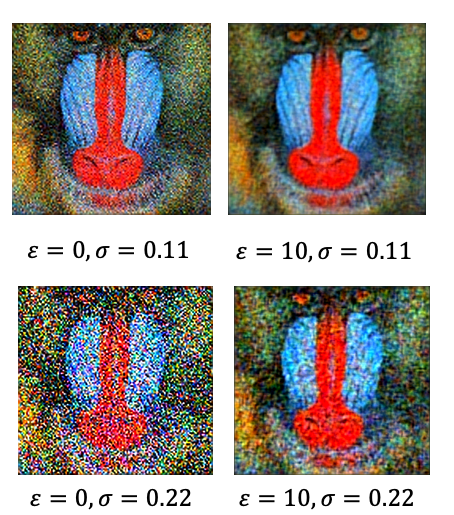
\includegraphics[width=8cm]{figures/epsball_qualitative_comp}
	\caption{Qualitative comparison between the impact of perturbation on a
  model trained without and with $\epsilon$-ball (scale = 4, dataset = SET14).}
  \label{fig:epsball_qualitative_comp}
\end{figure}

In the following experiment the same model (\textit{aetad})\footnote{An overview over all model architectures can be found in the appendix.} was trained with different radii of the $\epsilon$-ball. It turns out that the right choice of $\epsilon$ is a trade-off between the reconstruction performance and robustness against perturbations, comp. \myfigref{fig:epsball_perturbation}.

\begin{figure}[!htbp]
	\centering
	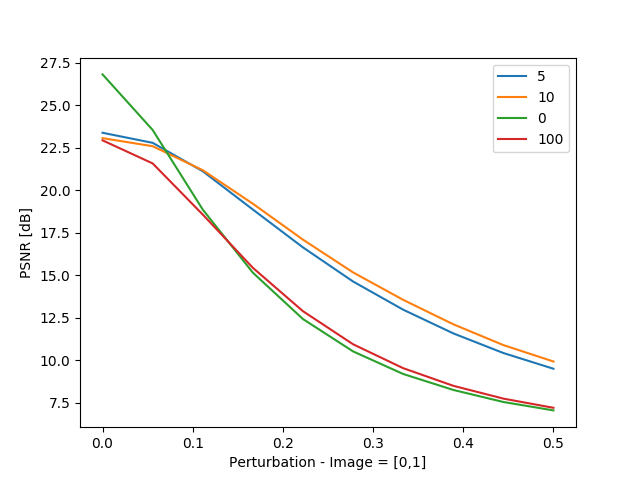
\includegraphics[width=10cm]{figures/epsball_perturbation}
	\caption{Reconstruction performance over several values of $\epsilon$
  and $\sigma$ (scale = 4).}
  \label{fig:epsball_perturbation}
\end{figure}

Also an increasing $\epsilon$ improves the convergence rate during training, as shown in \myfigref{fig:epsball_loss}, the model otherwise first overfits to $X_{GD}$ and then eventually finds a more optimal trade-off between fitting the low- and high-dimensional image (with increasing loss $\frac{\alpha}{\beta}$ ratio). However, as \myfigref{fig:epsball_perturbation} the radius of the $\epsilon$-ball
around $X_{GD}$ cannot be choosen infinitely large, since the overall performance worsens as the impact of the guidance image on the model convergence decreases (e.g. $\epsilon = 100$ in \myfigref{fig:epsball_perturbation}).

\begin{figure}[!htbp]
\centering
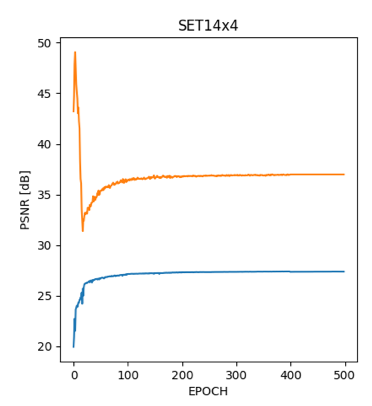
\includegraphics[width=6cm]{figures/epsball_loss_0_set14}
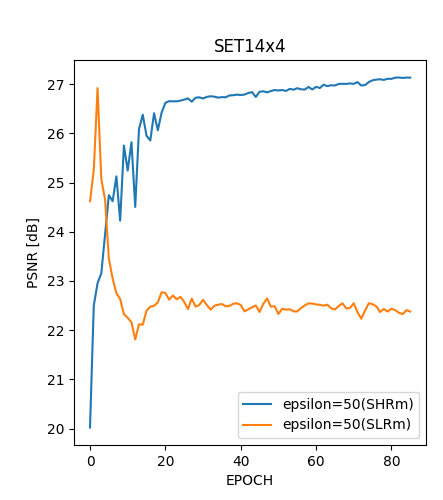
\includegraphics[width=6cm]{figures/epsball_loss_50_set14}
\caption{Closeness between $X_{SLR}$ and guidance image (blue) and $X_{SHR}$ and groudtruth image (orange) for different values of $\epsilon$ (left: $\epsilon = 1$, right $\epsilon = 50$) over number of epochs (pay attention to different convergence speed due to different scaling of number of epochs).}
\label{fig:epsball_loss}
\end{figure}

\mytableref{table:epsilonotherscales} displays the impact of models trained with different values of $\epsilon$ on the reconstruction capabilities on non-trained scales. In general the model overfits on a scale it is trained on, however allowing to deviate from the guidance image by increasing $\epsilon$ amplifies the effect of overfitting the learned transformation to a the scaling factor the model is trained on. Hence, as shown below especially for large deviations in scaling factor the accuracy worsens with increasing $\epsilon$.

\begin{table}[!htbp]
	\begin{center}
	\begin{tabular}{c|c|c|c|c}
	epsilon & x2 & x4 & x8 & x16 \\
	\hline
	0 & 8.446 & 24.406 & 8.555 & 18.938 \\
	20 & 6.244 & 22.188 & 6.492 & 17.308 \\
	50 & 6.771 & 22.459 & 6.925 & 16.992 \\
	100 & 10.901 & 23.784 & 11.870 & 13.225 \\
	\end{tabular}
	\caption{Impact of $\epsilon$ on performance on non-trained scales
	(trained scale = 4, dataset = SET14).}
	\label{table:epsilonotherscales}
	\end{center}
\end{table}

Overall the choice of $\epsilon$ depends very much on the application and its external conditions that should be solved, e.g. whether perturbations are probable for example during the storing, downloading etc. process.
In case only the performance without any disturbances matters, $\epsilon < 10$ is a good choice, as it fastens convergence of the model, prevents overfitting on the guidance image but also does not affect the accuracy without any disturbances much. For the further experiments a value $\epsilon = 1$ was used.
\newline
Although described for the \ac{SISR} problem here the described impact of
the $\epsilon$-ball is similar over all other problems, which omitted here for the matter of compactness of this report.

\section{Single-Image Super-Resolution}
\label{sec:Experiments_SISR}
Next to improving the robustness of the \ac{TAD} model several improvements were made on both the way of training as well as on the architecture itself. \myfigref{fig:psnr_complexity_sisr} shows the correlation on both the SET5 and the SET14 dataset for different architectures which were trained using the same parameters (learning parameters as described above, $\epsilon = 10$) for the sake of a comparability.

\begin{figure}[!htbp]
	\centering
	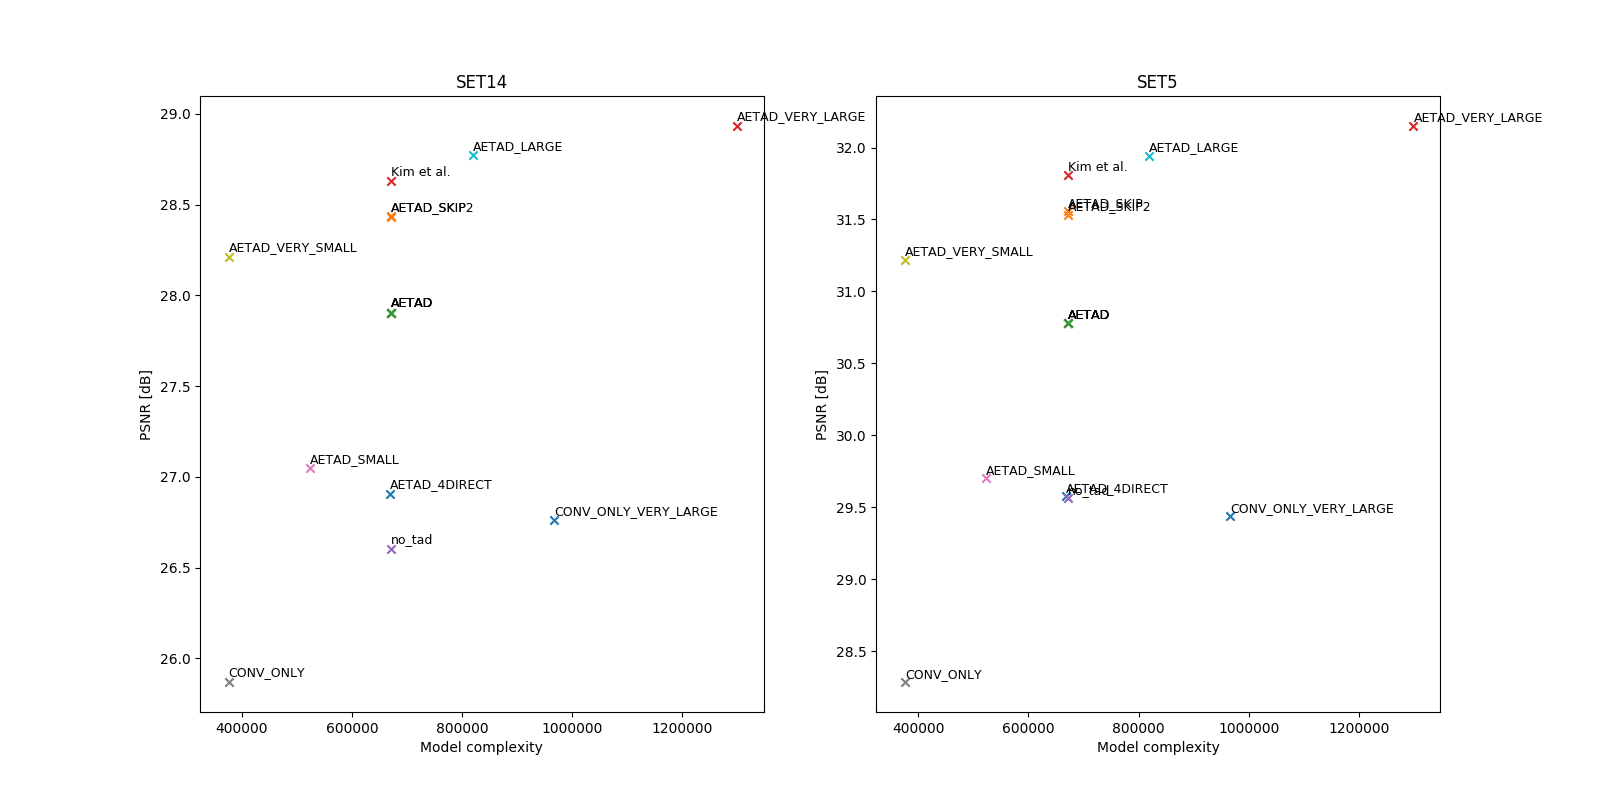
\includegraphics[width=18cm]{figures/psnr_complexity_sisr}
	\caption{Model complexity vs reconstruction performance for \ac{SISR}
	problem (scale = 4, dataset = SET14 and SET5).}
  \label{fig:psnr_complexity_sisr}
\end{figure}

Several conclusion can be drawn from \myfigref{fig:psnr_complexity_sisr}, which could be confirmed also for the other validation datasets used:

\begin{itemize}

\item The model \textit{no\_tad} is the baseline model which is trained to only upscale based on the guidance image, i.e. the standard approach to solve the \ac{SISR} problem. Although the reconstruction performance of the \textit{no\_tad} model is worse than state-of-the-art methods (e.g. VDSR \cite{AISRUVDCN} shown in \myfigref{fig:vdsr}), clearly the task-aware downscaling approach could largely improve the performance, compared the equivalent \textit{aetad} model which is trained using task aware downscaling. In fact for similar performance more than about $25 \%$ of the model parameters can be omitted, still resulting in a better accuracy (comparison \textit{no\_tad} vs \textit{aetad\_small}).

\item The \textit{Resblocks} have a large impact on the models performance, purely convolutional models with neither a skip connection nor a ReLU layer (as occurring in \textit{Resblocks}), such as the models \textit{conv\_only} or \textit{conv\_only\_very\_large}, have an overall worse reconstruction performance with a similar number of parameters.

\item In a direct comparison the model \textit{aetad\_direct4} performs worse than the iteratively scaling structured, but otherwise equivalent model \textit{aetad}.

\item In both displayed validation datasets the reconstruction performance stagnates with increasing number of parameters, as the difference in \ac{PSNR} between the \textit{aetad\_large} and the \textit{aetad\_very\_large} model does not improve much anymore.
\end{itemize}

\begin{table}[!htbp]
    \begin{center}
    \footnotesize
    \begin{tabular}{p{2cm}|p{2cm}|p{2cm}|p{3cm}|p{3cm}|p{3cm}}
    dataset & \pbox{2cm}{PSNR \\(Kim et al.)}
    & \pbox{2cm}{PSNR \\ (\textit{aetad\_skip2})}
    & \pbox{3cm}{\# model param. gain \\ (\textit{aetad\_skip2})}
    & \pbox{3cm}{PSNR \\ (\textit{aetad\_very\_small})}
    & \pbox{3cm}{\# model param. gain \\ (\textit{aetad\_very\_small})} \\
    \hline
    SET5 & 31.81 & 31.814 & 0 \% & 31.102 & -44 \% \\
    SET14 & 28.63 & 28.665 & 0 \% & 28.334 & -44 \% \\
    URBAN100 & 26.63 & 24.156 & 0 \% & 23.084 & -44 \% \\
    BSDS100 & 28.51 & 28.601 & 0 \% & 25.719 & -44 \% \\
    \end{tabular}
    \caption{Comparison of reconstruction accuracy between Kim et al. \cite{TAID},
    \textit{aetad\_skip2} and \textit{aetad\_very\_small}
    model for scaling factor 4 on several validation datasets. }
    \label{table:sisperformance}
    \normalsize
    \end{center}
\end{table}

While more complex architectures than the baseline (\textit{Kim et al.}-model) do not gain a lot of accuracy, for less complex models with similar architecture there is a large drop in accuracy. Therefore, the baseline architecture already is very reasonable. However, as shown in \myfigref{fig:psnr_complexity_sisr} and \myfigref{fig:sisr_models_architecture} a slight modification in the network structure which is adding another skip connection can lead to little improvements in reconstruction accuracy while having the same model complexity (\textit{aetad\_skip2}). Also the number of network parameters can be reduced by $44 \%$ by using only one \textit{Resblock} and convolutional layer with less filters while still having similar performance as the baseline model on the validation datasets shown (\textit{aetad\_very\_small}). \mytableref{table:sisperformance} gives an inside in the performance of the models pointed out in other standard validation datasets, such as URBAN100 and BSDS100. While the \textit{aetad\_skip2} model outperforms the baseline model in most datasets, the loose in performance between the baselines and the \textit{aetad\_skip2} model is larger on URBAN100 and BSDS100. This heviour predominantly has three reasons: First the validation dataset SET5 and SET14 are more similar to the training dataset DIV2K, second both datasets contain more images than SET5 and SET14 while the PSNR value is average over the PSNRs of each image. When one image is reconstructed very inaccurately, it highly affects the overall PSNR mean value. Besides, the model optimization process dominantly was based on the SET5 and SET14 dataset. 

\begin{figure}[!htbp]
    \centering
    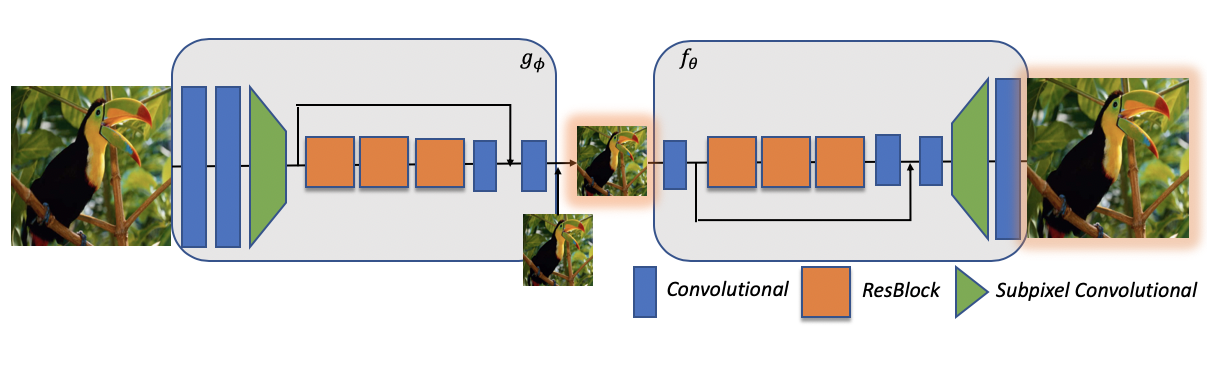
\includegraphics[width=12cm]{figures/architecture_baseline.png}
    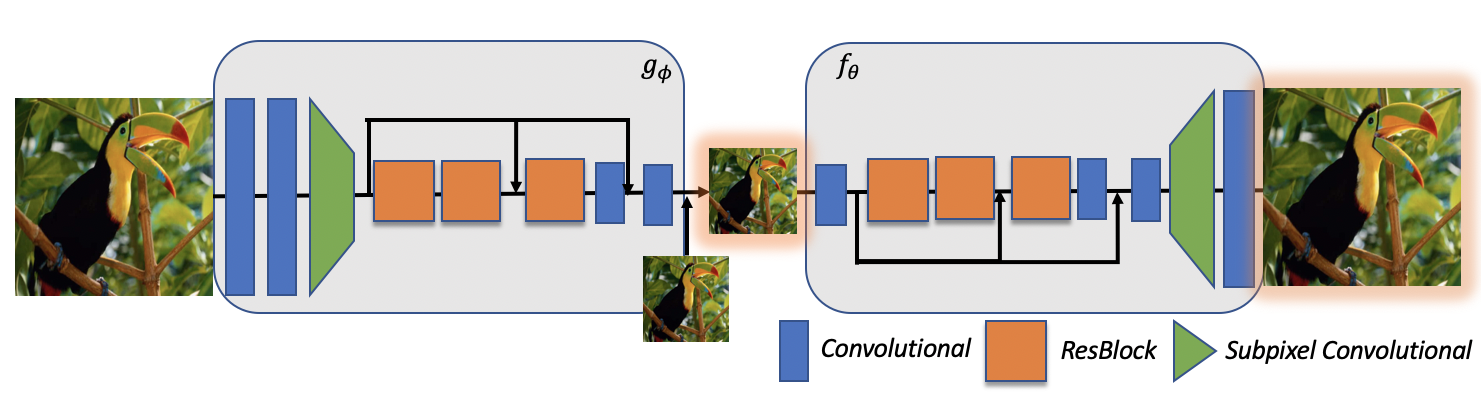
\includegraphics[width=12cm]{figures/architecture_skip2.png}
    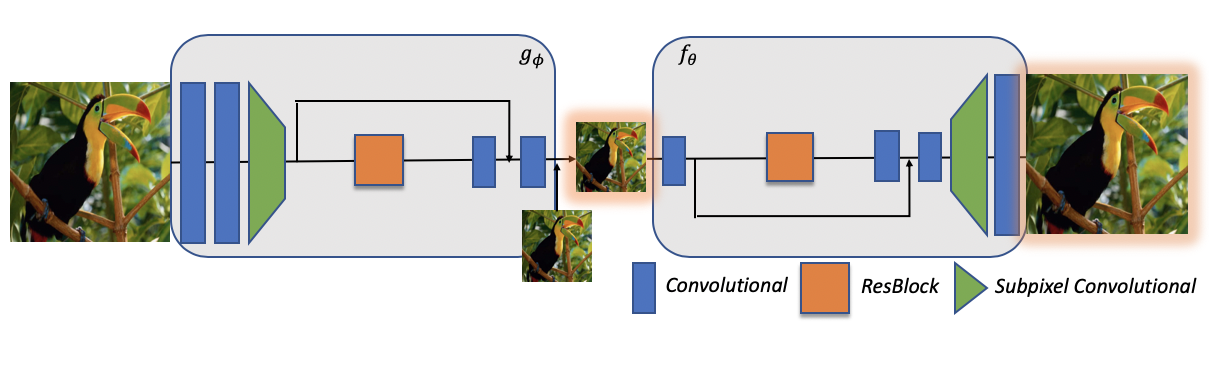
\includegraphics[width=12cm]{figures/architecture_very_small.png}
    \caption{Architectures of \textit{aetad\_skip2} (lower left) and \textit{aetad\_very\_small} (lower right) models in comparison to baseline model (upper).}
    \label{fig:sisr_models_architecture}
\end{figure}

\subsection*{Non-Trained Scaling Factors}
Having shown that \ac{TAD} can improve the reconstruction quality on the scaling factor it was trained on, in the following the performance on non-trained scales will be discussed. As shown in \mytableref{table:sisrotherscales} a model which upscales based on a bicubicly interpolated image (\textit{no\_tad}) performs better on other non-trained scale factors as the models using \ac{TAD}. This especially holds for large models as they overfit more to the learned transformation between low to high dimension. Therefore, although reconstructing best at the trained scaling factor $4$ the \textit{aetad\_very\_large} has the lowest \ac{PSNR} vale for other scaling factors (out of the compared models below). 

\begin{table}[!htbp]
    \begin{center}
    \begin{tabular}{c|c|c|c|c}
    model & x2 & x4 & x8 & x16 \\
    \hline
    \textit{no\_tad} & 7.457 & 27.204 & 7.459 & 19.488 \\
    \textit{aetad\_very\_small} & 8.527 & 28.334 & 7.780 & 18.799 \\
    \textit{aetad\_very\_large} & 5.882 & 28.935 & 5.928 & 18.673 \\
    \end{tabular}
    \caption{Comparison of the reconstruction performance on non-trained scales between task aware and non task aware trained models on SET14 (trained scale = 4).}
    \label{table:sisrotherscales}
    \end{center}
\end{table}

\subsection*{Large Scaling Factors}
Next to the scaling factor $4$ the performance of the chosen models on scaling factors have been explored.\footnote{As Kim et al. \cite{TAID} focused on expanding the approach to other scaling factors validating the models for large scaling factors was not prioritized in this work.}, up to 16. Exemplary in \mytableref{table:sisperformance_16} the performance of the \textit{aetad\_skip2} model on scaling factor 16 is displayed. Since there are no baseline data it is compared with bicubic upscaling. 

\begin{table}[!htbp]
    \begin{center}
    \begin{tabular}{c|c|c}
    dataset & PSNR (bicubic) & PSNR (\textit{aetad\_skip2})\\
    \hline
    SET5 & 19.137 & 20.982 \\
    SET14 & 18.669 & 20.038 \\
    VDIV2K & 20.920 & 23.209 \\
    \end{tabular}
    \caption{Comparison of reconstruction accuracy between chosen model and bicubicly interpolated baseline for scaling factor 16 on several validation datasets. }
    \label{table:sisperformance_16}
    \end{center}
\end{table}

\begin{figure}[!htbp]
	\centering
	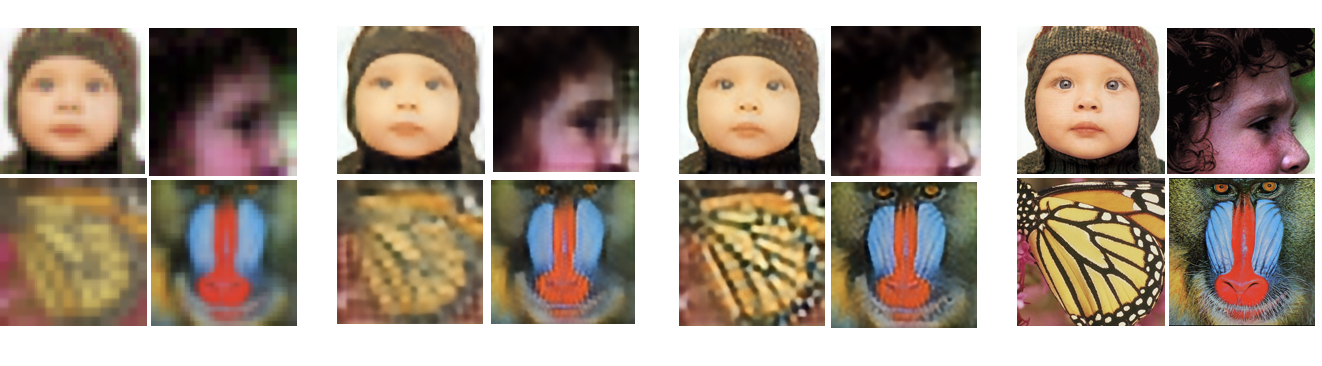
\includegraphics[width=16cm]{figures/examples_sisr_16.png}
	\caption{Examples of image reconstructions on SET5 data with scaling factor $16$ (from left to right: low-resolution, bicubicly upscaled, reconstructed and groundtruth image). }
  \label{fig:examples_sisr_16}
\end{figure}

\section{Video Super-Resolution}
\label{sec:Experiments_VSR}
This work is the first one applying \ac{TAD} in combination with the \ac{VSR} problem. Therefore, as a baseline the same \ac{VSR} model was trained to upscale bicubicly downscaled images (instead of task aware downscaled images), next to the upscaling each image individually using a \ac{SISR} model. The following table shows the reconstruction accuracy on the Vid4 validation dataset on both, the scaling factor $2$ and $4$.
\newline 
As displayed task aware downscaling clearly can improve the performance of the \ac{VSR} model that was used, since the \textit{task aware SOFVSR} model outperforms the \textit{SOFVSR} model that was trained non task aware for both scales, on every dataset. However, the \textit{SOFVSR} approach had to be re-implemented and was not tweaked much, as the goal of the project was to proof the feasibility of applying \ac{TAD} on the \ac{VSR} problem, so that even though the video super-resolution models are better than bicubicly upscaled low-dimensional frames for a scaling factor larger than $2$ the (tuned) single-image super-resolution model returns more accurately upscaled frames. 

\begin{table}[!htbp]
    \begin{center}
    \begin{tabular}{c|c|c|c|c|c}
    scale & dataset & Bicubic & \ac{SISR} model & non task aware SOFVSR
    & task aware SOFVSR \\
    \hline
    x2 & WALK & 24.224 & 29.523 & 26.215  & 30.433 \\
    x2 & FOLIAGE & 21.771 & 25.332 & 25.122 & 26.620 \\
    x4 & CALENDAR & 18.537 & 21.297 & 18.573  & 19.190 \\
    x4 & CITY & 23.483 & 25.332 & 24.191 & 24.677 \\
    \end{tabular}
    \caption{Comparison of reconstruction accuracy of bicubic interpolation, \ac{SISR} model as well as the rebuild SOFVSR model without and with \ac{TAD}.}
    \label{table:vsrperformance}
    \end{center}
\end{table}

\begin{figure}[!htbp]
	\centering
	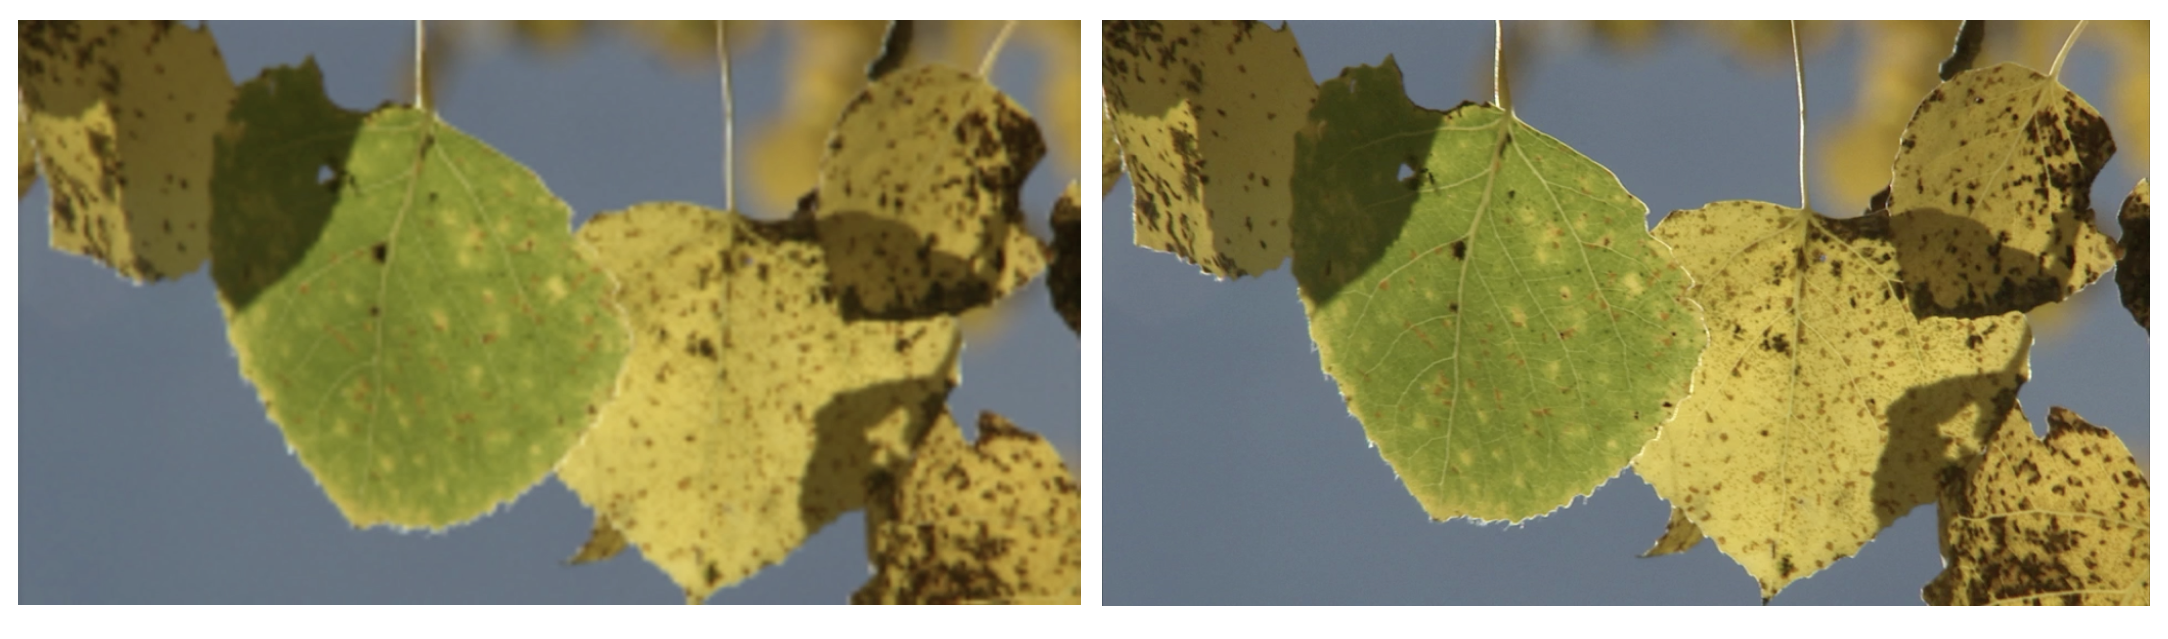
\includegraphics[width=16cm]{figures/examples_vsr_4.png}
	\caption{Examples of video-frame reconstructions on NTIAASPEN data with scaling factor $4$ (from left to right: bicubicly upscaled and reconstructed frame). Pay attention to the different levels of sharpness of the edges of the leafs. }
  \label{fig:examples_vsr_4}
\end{figure}

\section{Image Colorization}
\label{sec:Experiments_IC}
Similarly to the \ac{SISR} task in order to find a better accuracy (PSNR) - runtime (\# model parameters) - tradeoff several model architecture were tried, next to enhancing the training procedure as described in the introduction of \mysecref{sec:ExperimentsandResults}. The results are shown in \myfigref{fig:psnr_complexity_ic}. 

\begin{figure}[!htbp]
	\centering
	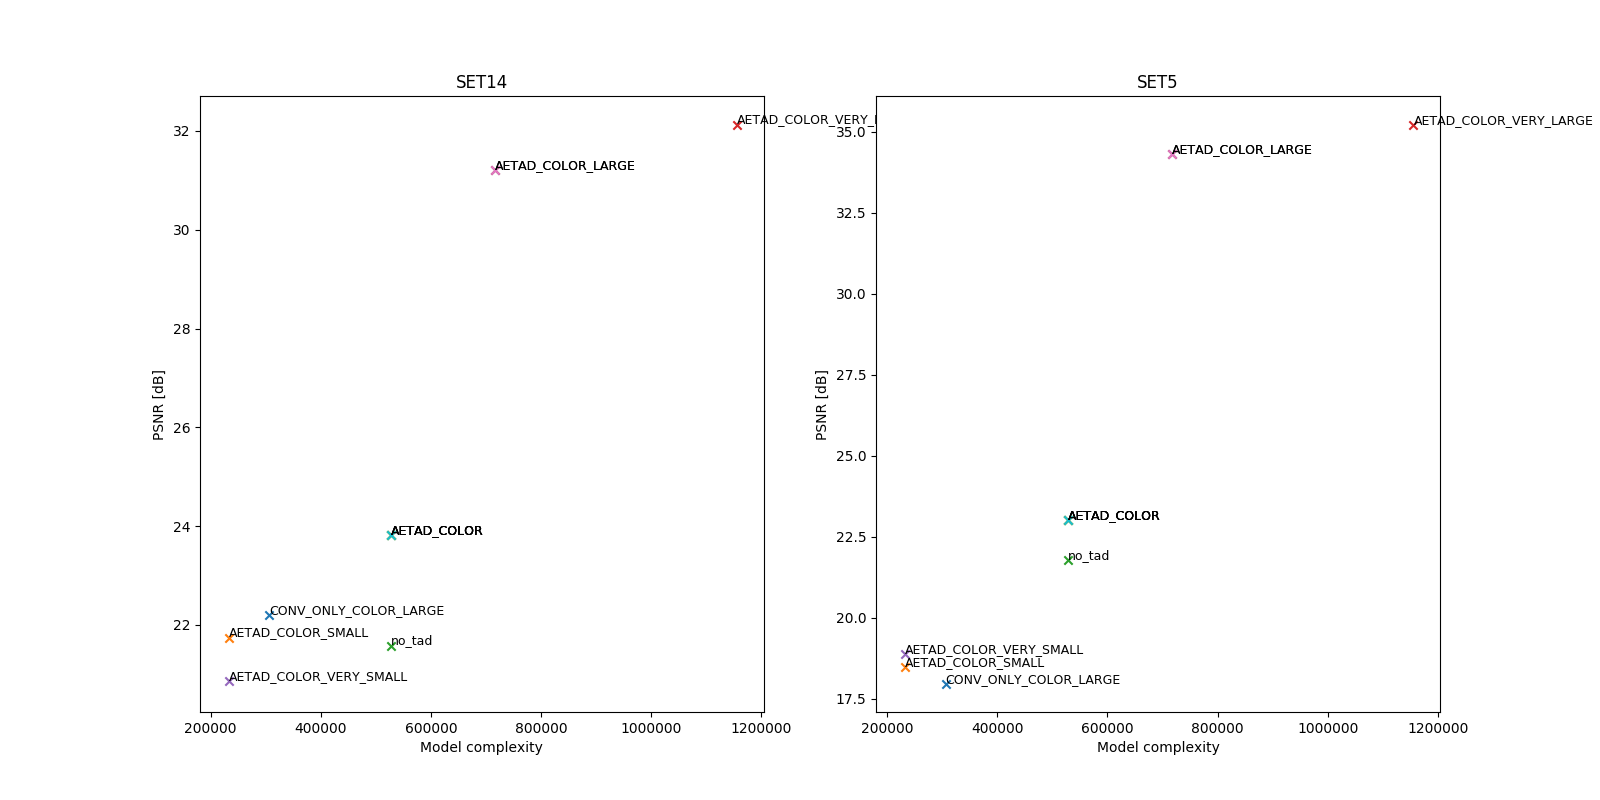
\includegraphics[width=18cm]{figures/psnr_complexity_ic}
	\caption{Model complexity vs reconstruction performance for \ac{IC}
	problem (dataset = SET14 and SET5).}
  \label{fig:psnr_complexity_ic}
\end{figure}

In opposite to \ac{SISR} here an increased model complexity results in a much better performance (\textit{aetad\_color\_large}), especially for the validation sets SET5 and SET14.\footnote{Kim et al. \cite{TAID} merely state a performance measure of their model for the BSDS100 and URBAN100 dataset, not for SET5 and SET14. Also they did not explicitly describe the model used for the \ac{IC} task, but claim it similar to the model they used (and described) for the \ac{SISR} task. Therefore, their model was re-implemeted and retrained, having similar results on URBAN100 and BSDS100, so that it is assumed to also perform similarly on SET5 and SET14. } 

\begin{table}[!htbp]
	\begin{center}
	\begin{tabular}{c|c|c|c}
	dataset & PSNR (Kim et al.) & PSNR (\textit{aetad\_color\_large})
	& \# model param. gain \\
	\hline
    SET5 & 22.56 & 34.416 & 35.7 \%\\
	SET14 & 23.78 & 31.262 & 35.7 \% \\
	URBAN100 & 33.68 & 33.604 & 35.7 \% \\
	BSDS100 & 36.14 & 36.786 & 35.7 \% \\
	\end{tabular}
	\caption{Comparison of reconstruction accuracy between Kim et al. \cite{TAID}, \textit{aetad\_color\_large} model on several validation datasets. }
	\label{table:icperformance}
	\end{center}
\end{table}

For deriving the \textit{aetad\_color\_large} model from the baseline model a \textit{Resblock} was added to both the decoder and encoder as well as the convolutional layer structure was changed (stepwise downscaling of number of filters, apportioned among two instead of one convolutional layer). 

\begin{figure}[!htbp]
	\centering
	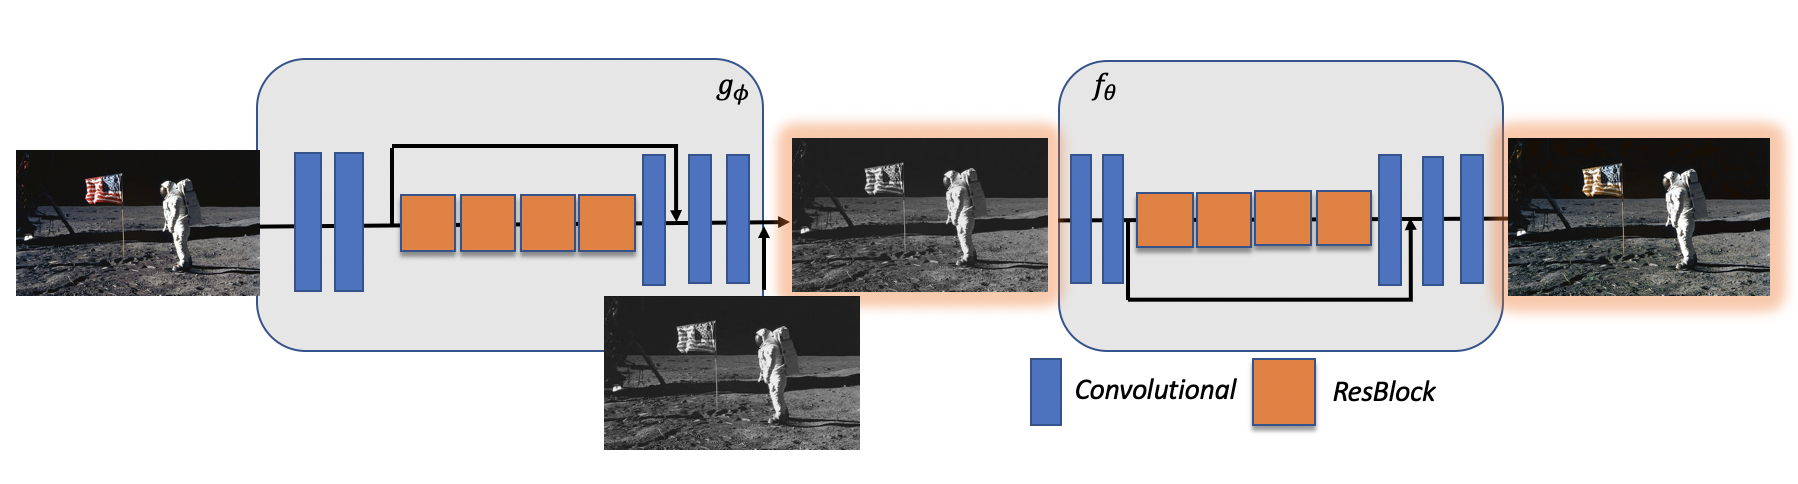
\includegraphics[width=12cm]{figures/architecture_color_large.png}
	\caption{Architectures of \textit{aetad\_color\_large} model (baseline model architecture  similar to \myfigref{fig:sisr_models_architecture}(upper).}
  \label{fig:final_model_ic}
\end{figure}

\begin{figure}[!htbp]
	\centering
	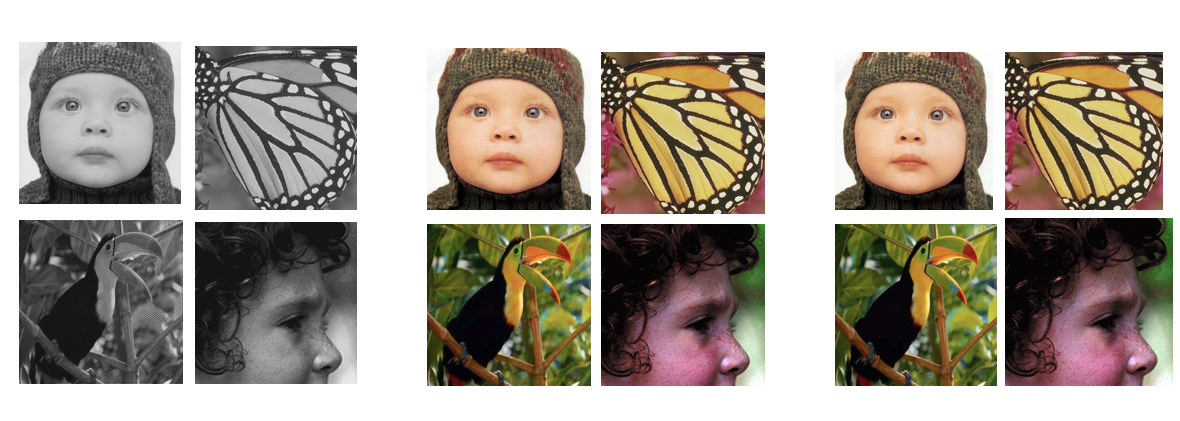
\includegraphics[width=16cm]{figures/examples_ic.png}
	\caption{Examples of color reconstructions on SET5 data using \textit{aetad\_color\_large} model (from left to right: grayscale, reconstructed and groundtruth image). }
  \label{fig:examples_ic}
\end{figure}

\section{Task Aware Low-Dimensional Image}
In the following the task aware low-dimensional image will be regarded more closely, by looking at artifacts that may occur (in comparison to trivially, non task aware downscaling) as well as at the resulting size of the low-dimensional representation compared to other compression algorithms such as jpg. 

\subsection*{Artifacts}
\myfigref{fig:slr_artifacts} contrasts the non task aware low-dimensional image against the task aware low-dimensional image. While there merely is a marginal difference between both low-resoluted images the grayscale images differ in the high frequency patterns, which are occuring on the task aware grayscale image. In general, during the project it was observed that a better reconstruction performance usually comes along with the occurrence of these high frequency patterns in the low-dimensional image (and a corresponding smaller PSNR value between guidance and task aware downscaled image). However, since the goal task aware downscaling is to optimize reconstruction while still ensuring human readability of the low-dimensional representation (which surely is still given), this trade-off was resolved in favor of reconstruction performance within this project. 

\begin{figure}[!htbp]
	\centering
	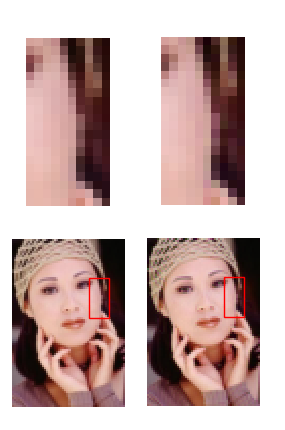
\includegraphics[width=6cm]{figures/sisr_slr_artifacts}
	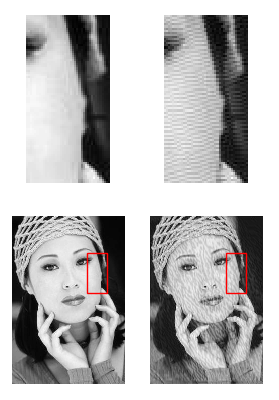
\includegraphics[width=6cm]{figures/ic_slr_artifacts}
	\caption{Low-dimensional image (SLR) artifacts for \ac{SISR} (left) and \ac{IC} (right) task, with trivially downscaled image at the left and task aware downscaling image at the right side of each pair.}
  \label{fig:slr_artifacts}
\end{figure}

\subsection*{Comparison to other Compression Algorithms}
To evaluate the shrinking performance of the \ac{TAD} in terms of the image size it was compared to the standard compression method jpeg \cite{jpeg} (using compression module from Mac OSX Mojave Preview application). As indicated in \mytableref{table:slr_size} for both the \ac{SISR} as well as the \ac{IC} task the algorithm outperforms jpeg in terms of compression rate. 

\begin{table}[!htbp]
	\begin{center}
	\begin{tabular}{c|c|c|c|c}
    & COL-png [KB] & COL-jpeg [KB] & SGRY [KB] & SLRx4 [KB] \\
    \hline
    baby & 365 & 286 & 191 & 32 \\ 
    bird & 119 & 112 & 66 & 11 \\
    butterfly & 130 & 110 & 56 & 10 \\
    head & 87 & 129 & 54 & 9 \\
    woman & 113 & 66 & 56 & 10 \\
	\end{tabular}
	\caption{Comparison of image size (KB) between groundtruth colorized image (COL-png), its jpeg-compression (COL-jpeg), the task aware downscaled grayscale image (SGRY) and the task aware downscaled low-resolution image for scaling factor $4$ (SLRx4) on SET5 dataset. }
	\label{table:slr_size}
	\end{center}
\end{table}

\section{Qualitative Improvements}
\label{sec:Experiments_QI}
As demonstrated above \ac{TAD} is able to improve the performance of
image reconstruction models quantitatively, but the \ac{TAD} approach also improves the results in a qualitative manner, in sense of that images can be restored that would be able to be restored from the trivially downscaled image, in the following shown using the example of a \ac{IC} task.
\newline
Consider \myfigref{fig:gummibears} displaying objects with equivalent shape but different colors (gummibears). While by using trivial downscaling methods like averaging over the colors (grayscale) some color information are irrecoverably lost, e.g. the yellow and orange gummibear looking nearly equivalent in grayscale, a task aware approach learns to keep basic color information despite of downscaling, figuratively speaking. Hence, even the color of shapes which are (exactly) similar in grayscale can be restored.

\begin{figure}[!htbp]
	\centering
	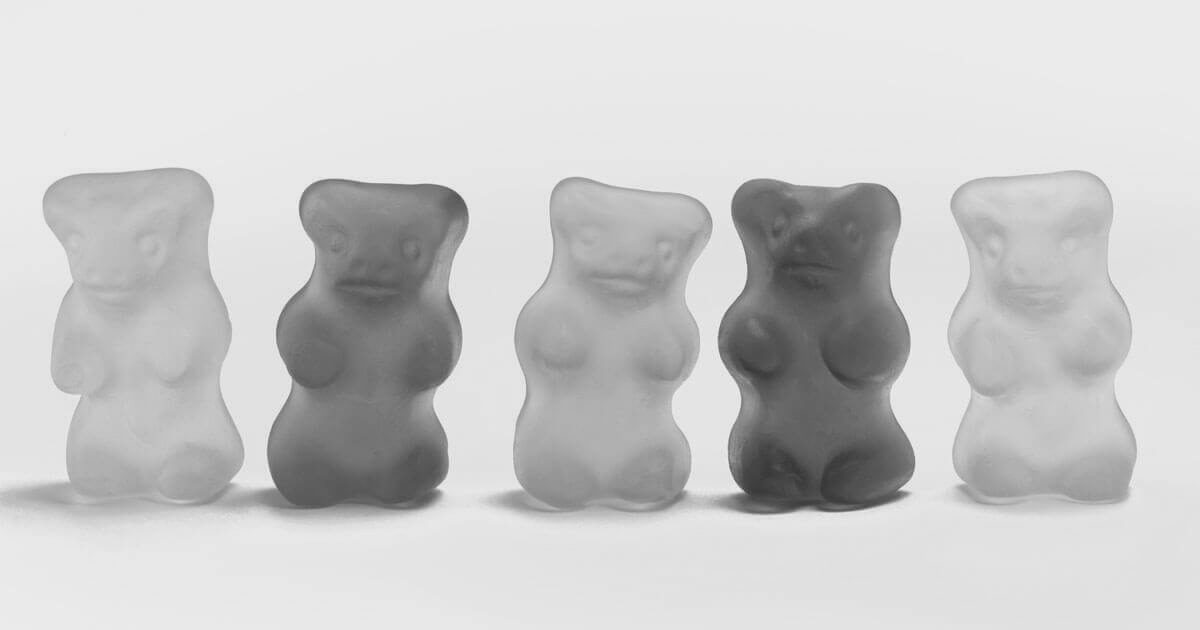
\includegraphics[width=8cm]{figures/gummibears_GRY}
	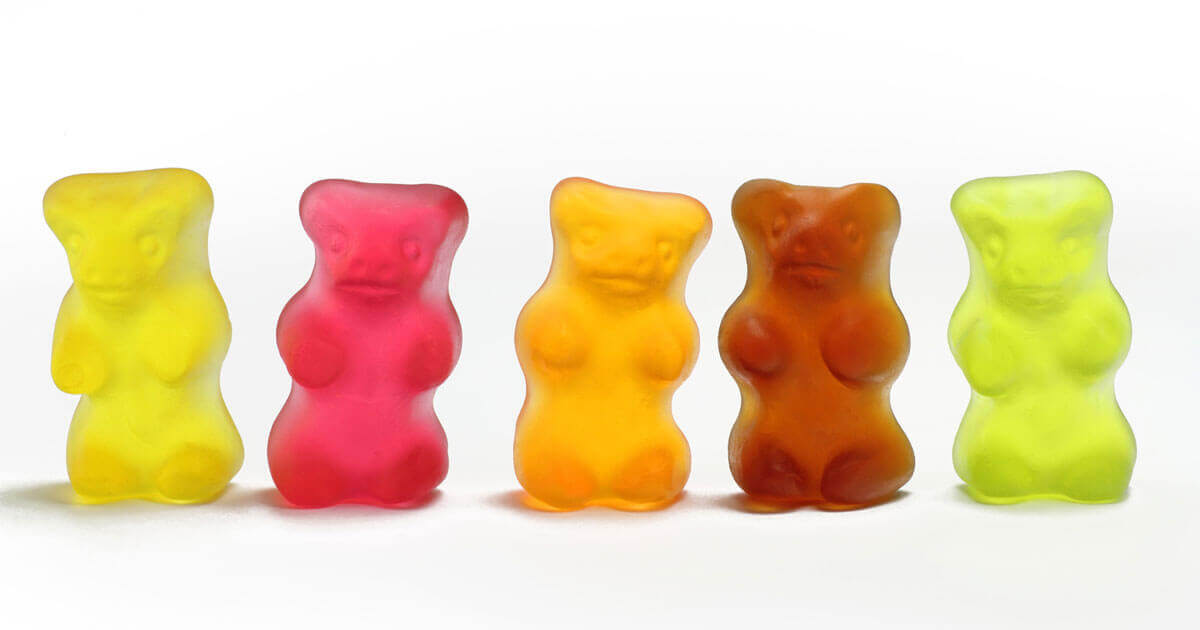
\includegraphics[width=8cm]{figures/gummibears_COL}
	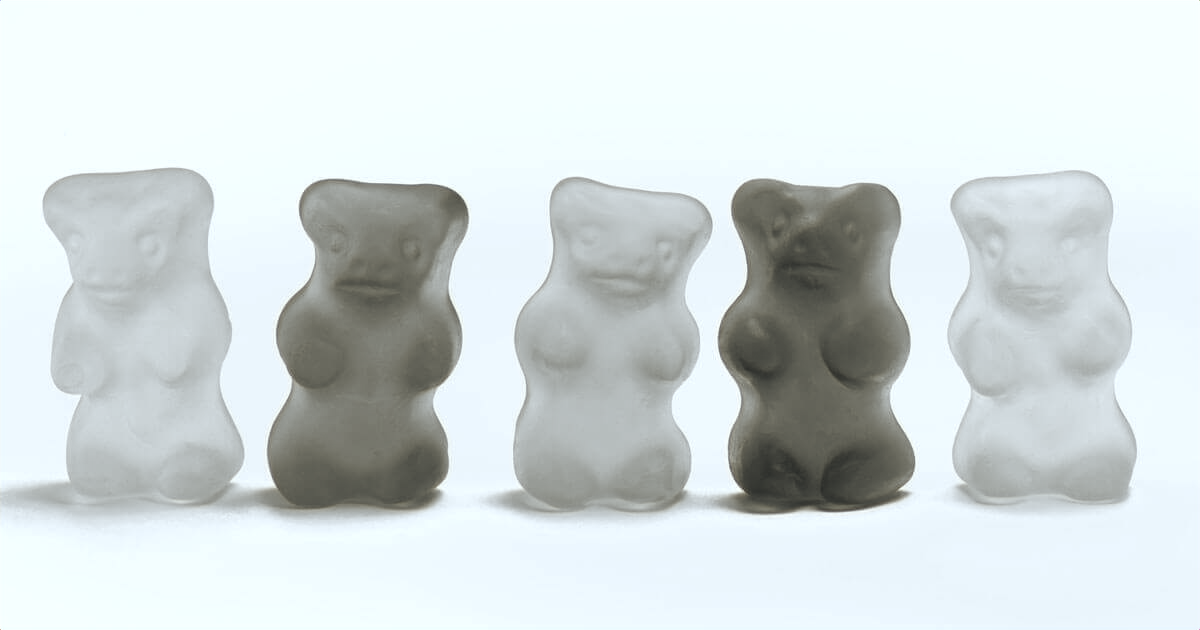
\includegraphics[width=8cm]{figures/gummibears_SCOLT_notad}
	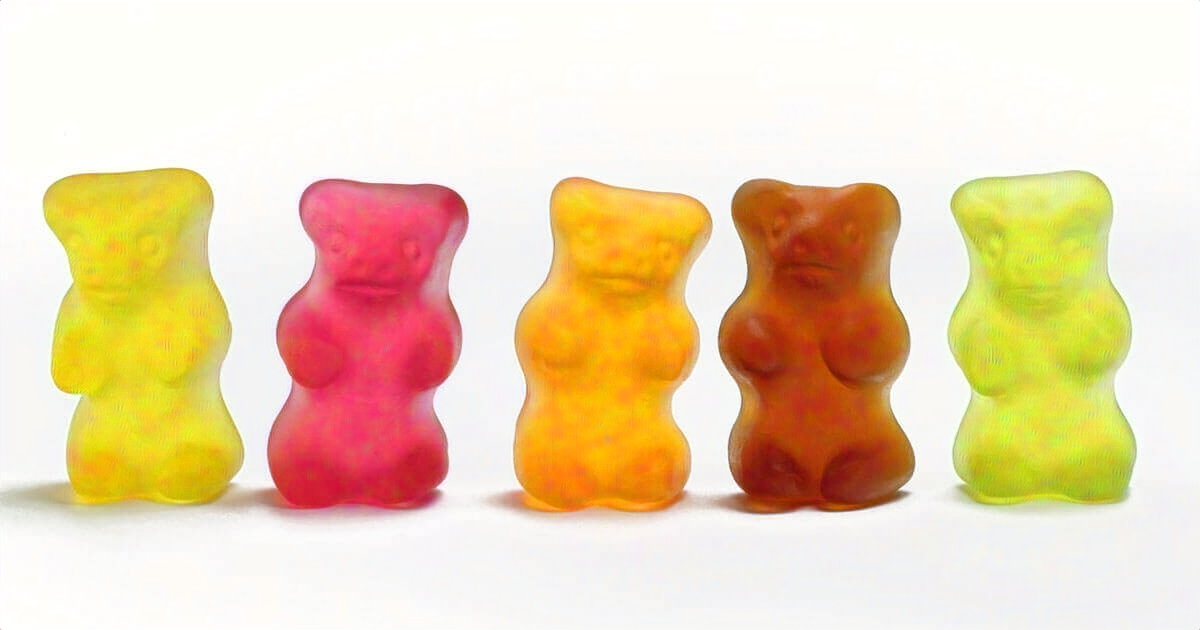
\includegraphics[width=8cm]{figures/gummibears_SCOLT}
	\caption{Image colorization of similar shapes (from upper left to lower
	right: grayscale, groundtruth, colorized without \ac{TAD}, colorized with \ac{TAD})}
  \label{fig:gummibears}
\end{figure}

% Describe the evaluation you did in a way, such that an independent researcher can repeat it. Cover the following questions:
% \begin{itemize}
%  \item \textit{What is the experimental setup and methodology?} Describe the setting of the experiments and give all the parameters in detail which you have used. Give a detailed account of how the experiment was conducted.
%  \item \textit{What are your results?} In this section, a \emph{clear description} of the results is given. If you produced lots of data, include only representative data here and put all results into the appendix.
% \end{itemize}
